% ============================================================
% Chapter 2 --- Metric, normed and inner-product spaces
% Originally: content/week-02.tex (Corsin Week 2, Monday) --- the hierarchy of structured
%             spaces and the metric axioms
%           + content/week-03.tex (Corsin Week 3, Friday) --- Cauchy--Schwarz and the
%             geometry of the inner product
% ============================================================
\chapter{Metric, Normed and Inner-Product Spaces}
\label{ch:metric_spaces}

% Transition: Claude Opus 5 (High)
% Corsin taught the two halves of this chapter a week apart, opening the later one with a recap
% of the definitions given here. sec:inner_products_recap keeps that recap, now as a pointer back
% to sec:structured_spaces rather than a repetition.
How much structure does a set need before one can do analysis on it? This chapter answers that by
taking $\mathbb{R}^n$ apart into layers. Distance comes first, and distance alone already carries
convergence and continuity. Adding a linear structure gives a norm, which measures the length of
one vector rather than the gap between two. Adding an inner product on top of that gives angles,
and with them orthogonal projection. The layers nest, each one strictly inside the last, and the
inequality that makes the innermost layer work at all is Cauchy--Schwarz. A last section settles
the question all of this raises: on $\mathbb{R}^n$ the choice of norm turns out not to matter for
anything topological, and it matters a great deal that this is a theorem rather than an
assumption.

% Originally: content/week-02.tex, \section{Structured spaces} (Corsin Week 2, Monday)

\section{Structured spaces}
\label{sec:structured_spaces}

This semester, you will be introduced to certain structures that can be given to a set, which in
this context is also called a \newterm{space} \germanfor{Raum} and which we will denote by $X$:

\begin{itemize}
  \item \textbf{0. Topological spaces:} fourth semester.
  % German mirror deliberately omitted here: this bullet is a preview, and the first *formal*
  % introduction of the term is \cref{def:metric_space}, which carries the \germanterm pair.
  \item \textbf{1. Metric spaces} $(X,\ d : X \times X \to \mathbb{R}_{\geq 0})$
    \begin{itemize}
      \item Defines a \textbf{distance} between points.
      \item $X$ is \textbf{not} necessarily a vector space.
      \item Covered in \textit{Analysis}.
    \end{itemize}
  \item \textbf{2. Normed metric spaces} $(X,\ \|\cdot\| : X \to \mathbb{R}_{\geq 0})$
    \begin{itemize}
      \item Defines the \textbf{length} of a vector.
      \item Presupposes a linear structure: $X$ must be a \textbf{vector space}.
      \item Covered in \textit{Linalg / Analysis}.
    \end{itemize}
  \item \textbf{3. Inner product spaces} $(X,\ \langle\cdot,\cdot\rangle : X \times X \to \mathbb{R})$
    \begin{itemize}
      \item Defines \textbf{both} lengths \textbf{and} angles!
      \item Super important!
      \item Covered in \textit{Linalg} (and sometimes used in \textit{Analysis}). $X$ is a \textbf{vector space}.
    \end{itemize}
\end{itemize}

\begin{center}
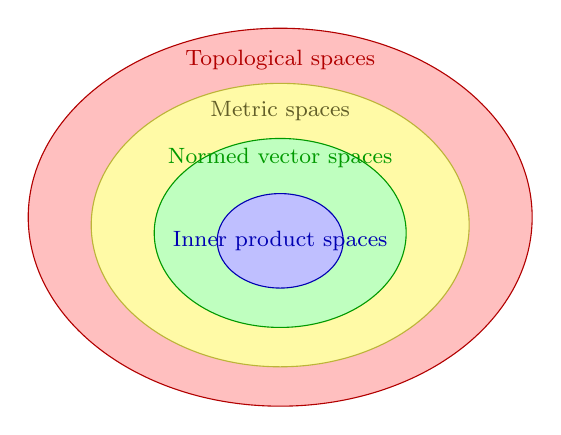
\begin{tikzpicture}
\fill[red!25] (0,0) ellipse (3.2 and 2.4);
\fill[yellow!35] (0,-0.1) ellipse (2.4 and 1.8);
\fill[green!25] (0,-0.2) ellipse (1.6 and 1.2);
\fill[blue!25] (0,-0.3) ellipse (0.8 and 0.6);
\draw[red!70!black] (0,0) ellipse (3.2 and 2.4);
\draw[yellow!70!black] (0,-0.1) ellipse (2.4 and 1.8);
\draw[green!60!black] (0,-0.2) ellipse (1.6 and 1.2);
\draw[blue!70!black] (0,-0.3) ellipse (0.8 and 0.6);
\node[red!70!black] at (0,2.0) {\footnotesize Topological spaces};
\node[olive!60!black] at (0,1.35) {\footnotesize Metric spaces};
\node[green!60!black] at (0,0.75) {\footnotesize Normed vector spaces};
\node[blue!70!black] at (0,-0.3) {\footnotesize Inner product spaces};
\end{tikzpicture}
\end{center}

You will see that an \textbf{inner product} $\langle\cdot,\cdot\rangle$ induces a \textbf{norm}
by the formula
\[\|x\| := \sqrt{\langle x, x\rangle}, \qquad x \in X.\]
Furthermore, a \textbf{norm} induces a \textbf{metric} by
\[d(x,y) := \|x - y\|, \qquad x, y \in X.\]

% Moved here from Week 3 (\S Cauchy--Schwarz): Corsin defines inner products and norms on the
% Friday of Week 3, but the two supplements below -- and the two displayed formulas above --
% already use both, so the definitions are stated here, at the point of first use. Corsin's own
% development of the geometry (angle, projection, the second proof of Cauchy--Schwarz) stays
% where he taught it, in \cref{sec:cauchy_schwarz}.
\begin{definition}[Inner product / scalar product]
\label{def:inner_product}
Let $V$ be a \textbf{vector space} over $\mathbb{R}$. An \newterm{inner product}
\germanfor{Skalarprodukt} on $V$ is a map
\[
\langle\cdot,\cdot\rangle : V \times V \to \mathbb{R}
\]
satisfying, for all $u, v, w \in V$ and $\alpha, \beta \in \mathbb{R}$:
\begin{enumerate}[label=\textbf{(\alph*)}]
  \item \textbf{Bilinearity:}
    $\langle \alpha u + \beta v, w\rangle = \alpha\langle u,w\rangle + \beta\langle v,w\rangle$,
    and equivalently in the second variable.
  \item \textbf{Symmetry:} $\langle u,v\rangle = \langle v,u\rangle$.
  \item \textbf{Definiteness:} $\langle u,u\rangle \geq 0$, and $\langle u,u\rangle = 0 \iff u = 0$.
\end{enumerate}
\end{definition}

\begin{definition}[Norm]
\label{def:norm}
Let $V$ be a \textbf{real} vector space. A \newterm{norm} \germanfor{Norm} on $V$ is a map
$\|\cdot\| : V \to [0,\infty)$ satisfying, for all $u, v \in V$ and $\alpha \in \mathbb{R}$:
\begin{enumerate}[label=\textbf{(\alph*)}]
  \item \textbf{Definiteness:} $\|v\| \geq 0$, and $\|v\| = 0 \iff v = 0$.
  \item \textbf{Homogeneity:} $\|\alpha v\| = |\alpha|\|v\|$.
  \item \textbf{$\Delta$-inequality:} $\|u+v\| \leq \|u\| + \|v\|$.
\end{enumerate}
\end{definition}

% Supplement: Analysis_II_Script_v1.pdf, p. 31
\begin{ainote}
The official script (Remark 9.94, p.\ 31 onward) adopts the opposite notational convention from
this document: from that point on \emph{it} writes the Euclidean norm as $|x|$ and reserves
$\|\cdot\|$ for non-standard norms. This document instead uses $\|\cdot\|$
(\texttt{\textbackslash lVert}\ldots\texttt{\textbackslash rVert}) uniformly for every norm,
Euclidean or not, per the house style, and keeps that convention throughout. Neither choice is
more standard than the other; this note exists only to warn anyone cross-referencing the script
directly that a bare $|\cdot|$ there and a bare $\|\cdot\|$ here can both denote \qt{the}
Euclidean norm. The warning matters most in the script's chapters 13--14, where the $|\cdot|$
convention is used densely.
\end{ainote}

% Source: Jérôme Paschoud/Notizen/Woche 4.1 Normen, das Differential.pdf, p. 1
% Generator: Gemini 3.1 Pro (High)
\begin{example}[Hilbert--Schmidt norm on matrix spaces]
\label{ex:hilbert_schmidt_norm}
A very important example of a norm on the space of real $n \times m$ matrices
$\mathbb{R}^{n \times m}$ is the \newterm{Hilbert--Schmidt norm} (also known as the Frobenius
norm). It is defined by
\[
\|M\|_2 := \sqrt{\Tr(M\transp M)},
\]
where $\Tr$ denotes the trace of a matrix. Only the diagonal of $M\transp M$ is needed, so the
off-diagonal entries are left unevaluated below. For a $2 \times 3$ matrix
$M = \left(\begin{smallmatrix} a & b & c \\ d & e & f \end{smallmatrix}\right)$, we have
\begin{align*}
M\transp M
  &= \begin{pmatrix} a & d \\ b & e \\ c & f \end{pmatrix}
     \begin{pmatrix} a & b & c \\ d & e & f \end{pmatrix} \\[0.6ex]
  &= \begin{pmatrix} a^2+d^2 & * & * \\ * & b^2+e^2 & * \\ * & * & c^2+f^2 \end{pmatrix}.
\end{align*}
The trace is the sum of the diagonal entries, so $\|M\|_2 = \sqrt{a^2+b^2+c^2+d^2+e^2+f^2}$. This
norm is therefore nothing but the standard Euclidean norm of the matrix entries read as a single
vector in $\mathbb{R}^{6}$, or in general in $\mathbb{R}^{nm}$. The inner product inducing it is
$\langle A, B \rangle := \Tr(A\transp B)$.
\end{example}

% Transition: Claude Opus 5 (High)
Comparing the three lists of axioms is already informative. A norm has exactly the three
properties a metric has, restated for a single vector instead of a pair of points, plus
homogeneity. That extra axiom has no metric analogue at all, since stating it requires scalar
multiplication. An inner product goes further and replaces the triangle inequality by
bilinearity, which is far stronger, and then recovers the triangle inequality as a \emph{theorem}
(\cref{prop:induced_norm_and_metric}) rather than assuming it. That is the precise sense in which
each layer carries more structure than the one outside it.

% The two blocks that follow supplement Corsin's outline with material from other tutors. They
% belong here logically, being about the innermost layer of the hierarchy just drawn, even though
% Corsin himself develops inner-product geometry only later (sec:cauchy_schwarz), where his own
% proof is kept. That prop:cauchy_schwarz_geometric_proof and thm:cauchy_schwarz are the same
% computation twice over is a mathematical point, and is made where it belongs, in
% rem:two_proofs_cauchy_schwarz.

% Supplement: Sascha Brack/Class Notes/Week_02_Notes_Monday_Updated.pdf, p. 4
\begin{remark}[Geometric angle and projection in inner product spaces]
\label{rem:inner_product_angle_geometry}
In an inner product space $(X, \langle\cdot,\cdot\rangle)$ over $\mathbb{R}$, the Cauchy--Schwarz inequality $|\langle x, y\rangle| \leq \|x\|\,\|y\|$ guarantees that for any non-zero vectors $x, y \in X$,
\[
-1 \leq \frac{\langle x, y\rangle}{\|x\|\,\|y\|} \leq 1.
\]
This allows us to formally define the \newterm{angle} $\Theta(x,y) \in [0,\pi]$ between $x$ and $y$ via
\[
\Theta(x,y) := \arccos\left(\frac{\langle x, y\rangle}{\|x\|\,\|y\|}\right).
\]
Geometrically, when $\|x\| = \|y\| = 1$, the inner product $\langle x, y\rangle$ is the signed
length of the orthogonal projection of $y$ onto the direction of $x$. In that reading
Cauchy--Schwarz becomes visually obvious: a projection of a unit vector cannot be longer than the
unit vector itself, so $\langle x,y\rangle \leq 1$, with equality exactly when $y$ already points
along $x$.
\begin{center}
% Generator: Claude Opus 5 (High) --- redrawn. The previous version parked a 6cm text block
% inside the picture, which pushed the figure off-centre and stated in words what the drawing
% should state by itself. Both vectors are unit, so they sit on the dashed unit circle; the
% angle arc now shows Theta, and the projection foot P = (cos 50, 0) is marked with a right
% angle. Angle 50 degrees: cos(50) = 0.643, sin(50) = 0.766.
\begin{tikzpicture}[>=Latex, scale=2.7]
  \coordinate (O) at (0,0);
  \coordinate (X) at (1,0);
  \coordinate (Y) at ({cos(50)},{sin(50)});
  \coordinate (P) at ({cos(50)},0);

  \draw[->, gray!55] (-0.18,0) -- (1.32,0);
  \draw[->, gray!55] (0,-0.18) -- (0,1.12);

  % both vectors are unit, so they end on this circle
  \draw[gray!40, dashed] (O) circle (1);

  % angle between x and y
  \draw[green!45!black, thick] (0.32,0) arc (0:50:0.32);
  \node[green!45!black, font=\footnotesize] at (0.50,0.17) {$\Theta$};

  % dropped perpendicular, with a right-angle mark at the foot
  \draw[blue!55, dashed] (Y) -- (P);
  \draw[blue!55] ({cos(50)-0.07},0) -- ({cos(50)-0.07},0.07) -- ({cos(50)},0.07);

  % The projection has to be measured BELOW the axis: drawn on the axis it would be collinear
  % with the arrow for x and simply disappear underneath it.
  \draw[orange!90!black, dotted] (0,0) -- (0,-0.17);
  \draw[orange!90!black, dotted] ({cos(50)},0) -- ({cos(50)},-0.17);
  \draw[orange!90!black, line width=0.9pt, <->] (0,-0.17) -- ({cos(50)},-0.17);
  \node[orange!90!black, font=\footnotesize, below] at ({cos(50)/2},-0.18)
    {$\langle x,y\rangle$};

  \draw[blue!60!black, thick, ->] (O) -- (X) node[above right, font=\small] {$x$};
  \draw[blue!60!black, thick, ->] (O) -- (Y) node[above left, font=\small] {$y$};

  \node[gray!55!black, font=\footnotesize, anchor=west] at (1.0,0.92) {$\|x\|=\|y\|=1$};
\end{tikzpicture}
\end{center}
\end{remark}

% Quelle: Diego Torres Tejeda/Notes - 09.03 - Diego Torres Tejeda.pdf, pp. 1--2
\begin{proposition}[Geometric derivation of the Cauchy--Schwarz inequality]
\label{prop:cauchy_schwarz_geometric_proof}
Let $(V, \langle\cdot,\cdot\rangle)$ be a real inner product space. Then for all $v, w \in V$,
\[
|\langle v, w\rangle| \leq \|v\|\,\|w\|.
\]
\end{proposition}

\begin{proof}
If $w = 0$, both sides vanish and the inequality holds trivially. For $w \neq 0$, consider the squared distance from $v$ to the points of the line $L := \operatorname{span}_{\mathbb{R}}\{w\}$, parametrized by $\lambda \mapsto \lambda w$:
\[
f(\lambda) := \|v - \lambda w\|^2 = \langle v - \lambda w, v - \lambda w\rangle = \|v\|^2 - 2\lambda\langle v, w\rangle + \lambda^2\|w\|^2.
\]
Since $f(\lambda) \geq 0$ for all $\lambda \in \mathbb{R}$, $f$ is a convex quadratic polynomial in $\lambda$ with positive leading coefficient $\|w\|^2 > 0$. Differentiating or completing the square shows that $f$ attains its global minimum at $\lambda_0 := \frac{\langle v, w\rangle}{\|w\|^2}$. Evaluating $f$ at $\lambda_0$ yields
\[
0 \leq f(\lambda_0) = \|v\|^2 - 2\frac{\langle v, w\rangle^2}{\|w\|^2} + \frac{\langle v, w\rangle^2}{\|w\|^2} = \|v\|^2 - \frac{\langle v, w\rangle^2}{\|w\|^2}.
\]
Multiplying by $\|w\|^2$ and taking square roots gives $|\langle v, w\rangle| \leq \|v\|\,\|w\|$. Geometrically, $\pi_L(v) := \lambda_0 w = \frac{\langle v, w\rangle}{\|w\|^2}w$ is the unique orthogonal projection of $v$ onto the line $L$, achieving the minimal distance $d(v, L) = \sqrt{f(\lambda_0)}$.
\end{proof}

% Generator: Claude Opus 5 (High) --- moved here from Week 3 together with \cref{def:norm}:
% Cauchy--Schwarz is now available (immediately above), which is the only input the triangle
% inequality needs, so the two arrows of the hierarchy can be justified where they are drawn.
\begin{proposition}[Inner product $\Rightarrow$ norm $\Rightarrow$ metric]
\label{prop:induced_norm_and_metric}
Let $V$ be a real vector space.
\begin{enumerate}[label=\textbf{(\alph*)}]
  \item If $\langle\cdot,\cdot\rangle$ is an inner product on $V$ (\cref{def:inner_product}),
    then $\|v\| := \sqrt{\langle v,v\rangle}$ is a norm on $V$ (\cref{def:norm}).
  \item If $\|\cdot\|$ is a norm on $V$, then $d(x,y) := \|x-y\|$ is a metric on $V$
    (\cref{def:metric_space}).
\end{enumerate}
\end{proposition}

\begin{proof}
\textbf{(a)} Definiteness of the norm is definiteness of the inner product, and homogeneity
follows from bilinearity: $\|\alpha v\|^2 = \langle\alpha v,\alpha v\rangle =
\alpha^2\|v\|^2$. For the triangle inequality, expand and apply
\cref{prop:cauchy_schwarz_geometric_proof}:
\begin{align*}
  \|u+v\|^2 &= \|u\|^2 + 2\langle u,v\rangle + \|v\|^2 \\
            &\leq \|u\|^2 + 2\lvert\langle u,v\rangle\rvert + \|v\|^2 \\
            &\leq \|u\|^2 + 2\|u\|\,\|v\| + \|v\|^2 \ =\ \big(\|u\|+\|v\|\big)^2,
\end{align*}
and taking square roots gives $\|u+v\| \leq \|u\|+\|v\|$.

\textbf{(b)} Definiteness: $d(x,y)=0$ means $\|x-y\|=0$, hence $x=y$. Symmetry: homogeneity
with $\alpha=-1$ gives $\|x-y\| = \|-(y-x)\| = \|y-x\|$. Triangle inequality: writing
$x-z = (x-y)+(y-z)$,
\[d(x,z) = \|(x-y)+(y-z)\| \leq \|x-y\| + \|y-z\| = d(x,y)+d(y,z). \qedhere\]
\end{proof}

\begin{remark}[Neither arrow reverses]
\label{rem:norm_not_from_inner_product}
The nesting drawn above is strict at both steps.
\begin{itemize}
  \item \textbf{Not every metric comes from a norm.} The discrete metric
    (\cref{ex:metric_examples}\textbf{(a)}) on a vector space cannot: a norm-induced metric
    satisfies $d(\alpha x, 0) = |\alpha|\,d(x,0)$, which fails as soon as
    $\alpha \neq 0,\pm1$.
  \item \textbf{Not every norm comes from an inner product.} A norm induced by an inner product
    obeys the \newterm{parallelogram law}
    $\|u+v\|^2 + \|u-v\|^2 = 2\|u\|^2 + 2\|v\|^2$ (expand both sides by bilinearity). The
    supremum norm on $\mathbb{R}^2$ violates it: for $u := (1,0)$ and $v := (0,1)$ the left side
    is $1+1 = 2$ and the right side is $2+2 = 4$.
\end{itemize}
Consequently, each layer of the hierarchy really does carry strictly more structure than the one
outside it. The picture at the start of this section is a genuine nesting of four distinct
classes, not a chain of equivalent descriptions of the same thing.
\end{remark}

% Source: Corsin Nick/Class Notes/Week 2.pdf, pp. 1--13

% Originally: content/week-02.tex, \section{Metric spaces} (Corsin Week 2, Monday)

\section{Metric spaces}
\label{sec:metric_spaces}

\begin{definition}[Metric space]
\label{def:metric_space}
A \newterm{metric space} (\germanterm{metrischer Raum}) $(X,d)$ is any set $X$ with a
\newterm{metric} (\germanterm{Metrik}) $d : X \times X \to \mathbb{R}_{\geq 0}$ such that for all
$x, y, z \in X$:
\begin{enumerate}[label=\textbf{(\alph*)}]
  \item \textbf{Definiteness:} $d(x,y) \geq 0$, with equality if and only if $x = y$. In words: the
    distance is non-negative, and a point has zero distance to itself.
  \item \textbf{Symmetry:} $d(x,y) = d(y,x)$, i.e., $x$ has the same distance to $y$ as $y$ to $x$.
  \item \textbf{Triangle inequality ($\Delta$-inequality):} $d(x,z) \leq d(x,y) + d(y,z)$ ---
    \qt{detours make the way longer}.
\end{enumerate}
\end{definition}

\begin{ainote}
Corsin's gloss on definiteness reads \qt{the distance positive}; the formula $d \geq 0$ is
correct, but the gloss omits the ``non-''. Corrected in the prose above.
\end{ainote}

\begin{center}
\begin{tikzpicture}[>=Latex]
\draw[->] (-0.3,0) -- (4.2,0);
\draw[->] (0,-0.3) -- (0,3);
\coordinate (x) at (0.2,0.2);
\coordinate (y) at (1.6,2.0);
\coordinate (z) at (3.6,2.3);
\draw[blue,thick,->] (x) -- (y);
\draw[blue,thick,->] (y) -- (z);
\draw[red,thick,->] (x) -- (z);
\fill (x) circle (1.5pt) node[below]{$x$};
\fill (y) circle (1.5pt) node[above]{$y$};
\fill (z) circle (1.5pt) node[above]{$z$};
\node[red] at (2.3,0.7) {\footnotesize $d(x,z)$};
\node[blue] at (0.6,1.3) {\footnotesize $d(x,y)$};
\node[blue] at (2.7,2.4) {\footnotesize $d(y,z)$};
\node[red,below] at (2,-0.6) {\small $d(x,z) \le d(x,y)+d(y,z)$};
\end{tikzpicture}
\end{center}

% Generator: Claude Opus 5 (Medium)
\begin{aiexample}[Each axiom rules out something, and none is redundant]
\label{ex:metric_axioms_are_needed}
Three functions on $\mathbb{R}$, each failing exactly one axiom of
\Cref{def:metric_space}. It is worth checking these once: a definition only becomes memorable
once you know what it is keeping out.
\begin{enumerate}[label=\textbf{(\alph*)}]
  \item \textbf{Definiteness fails:} $d(x,y) := |x^2-y^2|$. This is symmetric and satisfies the
    triangle inequality (it is $|\cdot|$ composed with $x \mapsto x^2$), but
    $d(-1,1) = 0$ while $-1 \neq 1$. Distinct points at distance zero: the space cannot tell
    $-1$ from $1$, and no sequence could ever have a unique limit.
  \item \textbf{Symmetry fails:} $d(x,y) := \max\{\,y-x,\ 2(x-y)\,\}$, i.e.\ moving to the right
    costs $1$ per unit and moving to the left costs $2$. Here $d(0,1)=1$ but $d(1,0)=2$, so the
    return trip is more expensive than the outward one. Definiteness still holds ---
    $d(x,y) = 0$ forces $y-x \leq 0 \leq y-x$, hence $x=y$ --- and so does the triangle
    inequality, since $d(x,y) = \varphi(y-x)$ for $\varphi(t) := \max\{t,-2t\}$, and $\varphi$
    is a maximum of two linear functions vanishing at $0$, hence convex and positively
    homogeneous, hence subadditive. (Such a $d$ is called a \newterm{quasi-metric} and is
    genuinely useful elsewhere --- but $B_r(x)$ would then depend on which argument the centre
    sits in.)
  \item \textbf{Triangle inequality fails:} $d(x,y) := (x-y)^2$. Definiteness and symmetry are
    clear, but
    \[d(0,2) = 4 \quad > \quad d(0,1)+d(1,2) = 1+1 = 2,\]
    so the detour through $1$ is \emph{shorter} than going direct --- exactly the
    \qt{detours make the way longer} slogan reversed.
\end{enumerate}
\end{aiexample}

\subsection{Examples}

% Transition: Claude Opus 5 (High)
Three axioms are few enough that a great many things qualify as metrics, and the point of the
list below is exactly that breadth. Two of the examples are not what one would draw on a
blackboard as \qt{distance}: the discrete metric measures nothing but \qt{same or different},
and the supremum metric measures the distance between two \emph{functions}. Both are legitimate,
and it is worth letting them stretch the intuition now --- the second, in particular, is the
setting in which uniform convergence turns out to be an ordinary case of
\cref{def:convergent_sequence} (\cref{ex:uniform_convergence}).

% Source: Corsin Nick/Class Notes/Week 2.pdf, pp. 1--13
\begin{example}[Standard metrics on $\mathbb{R}^n$]
\label{ex:metric_examples}
\begin{enumerate}[label=\textbf{(\alph*)}]
  \item Let $X$ be a set. The \newterm{discrete metric} is given by
    \[d(x,y) := \begin{cases} 1 & \text{if } x \neq y \\ 0 & \text{if } x = y \end{cases}\]
    Important for counterexamples!
  \item Let $X := \mathbb{R}^n$. Then we have many choices for a metric; some common ones are:
  \begin{enumerate}[label=\textbf{(\roman*)}]
    \item \textbf{Manhattan metric:}
      \[d_1(x,y) := |x_1 - y_1| + \dots + |x_n - y_n| = \sum_{k=1}^{n} |x_k - y_k|\]
    \item \textbf{Standard metric:}
      \[d_2(x,y) := \sqrt{(x_1-y_1)^2 + \dots + (x_n-y_n)^2} = \sqrt{\sum_{k=1}^{n}(x_k - y_k)^2}\]
    \item \textbf{Supremum metric:}
      \[d_3(x,y) := \sup_{k = 1,\dots,n} |x_k - y_k|\]
  \end{enumerate}
\end{enumerate}
\end{example}

\begin{center}
\begin{tikzpicture}[>=Latex, scale=1.1]
  \draw[->] (-0.3,0) -- (4.5,0) node[right] {$x_1$};
  \draw[->] (0,-0.3) -- (0,3.5) node[above] {$x_2$};
  \coordinate (X) at (0.8, 0.8);
  \coordinate (Y) at (3.8, 2.8);
  \coordinate (Corner) at (3.8, 0.8);

  \draw[dotted, gray] (0, 0.8) node[left, font=\footnotesize] {$x_2$} -- (X) -- (0.8, 0) node[below, font=\footnotesize] {$x_1$};
  \draw[dotted, gray] (0, 2.8) node[left, font=\footnotesize] {$y_2$} -- (Y) -- (3.8, 0) node[below, font=\footnotesize] {$y_1$};

  % The two legs are just coordinate differences -- neither one IS a metric.
  \draw[orange!90!black, ultra thick] (X) -- (Corner) -- (Y);
  \node[below, font=\small, orange!90!black] at (2.3,0.72) {$a := |x_1-y_1|$};
  \node[right, font=\small, orange!90!black] at (3.9,1.8) {$b := |x_2-y_2|$};

  \draw[blue!80!black, very thick] (X) -- (Y);
  \node[above left, font=\small, blue!80!black] at (2.9,2.1) {$d_2 = \sqrt{a^2+b^2}$};

  \fill (X) circle (2pt) node[above left] {$x$};
  \fill (Y) circle (2pt) node[above right] {$y$};

  % d_3 picks out the longer leg; here a > b.
  \draw[red!80!black, thick, <->] (0.8,-0.95) -- node[below, font=\small] {$d_3 = \max\{a,b\} = a$} (3.8,-0.95);
  \draw[red!80!black, dotted] (0.8,0) -- (0.8,-0.95);
  \draw[red!80!black, dotted] (3.8,0) -- (3.8,-0.95);

  \node[orange!90!black, font=\small, anchor=west] at (0.1,3.25) {$d_1 = a+b$ \ (the full orange path)};
\end{tikzpicture}
\end{center}

Note that $d_1$ is the \textbf{sum} of the two legs and $d_3$ the \textbf{larger} of them ---
neither is a single leg on its own. Only $d_2$ is the straight-line distance you would draw by
reflex.

In general,
\[
d(x,y) := \sqrt[m]{\sum_{k=1}^{n} (x_k - y_k)^m}
\]
is a metric on $\mathbb{R}^n$ for any $m$.

\begin{ainote}
Two caveats Corsin leaves out. The powers must be taken of \textbf{absolute values},
$\sqrt[m]{\sum_k|x_k-y_k|^m}$ --- otherwise for odd $m$ the radicand can be negative. And it is
a metric only for $m \geq 1$: for $m \in (0,1)$ the triangle inequality fails, as
\Cref{ex:4.3}\textbf{.6} shows with $x=e_1$, $y=e_2$, where
$|x+y|_m = 2^{1/m} > 2 = |x|_m+|y|_m$. Written as stated above.
\end{ainote}

\begin{example}[continued]
\begin{enumerate}[label=\textbf{(\alph*)}, start=3]
  \item Let $X := C^0([0,1], \mathbb{R})$ be the set of continuous functions $[0,1] \to \mathbb{R}$.
    Then we can define the \newterm{supremum metric} for $f, g \in X$:
    \[
    d(f,g) := \sup_{x \in [0,1]} |f(x) - g(x)|
    \]
    This is well defined --- i.e.\ the supremum is a real number and not $+\infty$ --- because
    $|f-g|$ is continuous on the compact interval $[0,1]$ and therefore bounded, by the extreme
    value theorem from \emph{Analysis I} (revisited in this generality as
    \cref{lem:sequential_compactness_extreme_values} below). Compactness of the domain is doing
    real work here: on $C^0(\mathbb{R},\mathbb{R})$ the same formula would produce $\infty$ for
    $f(x) := x$, $g := 0$.
  \item Let $X := S^2 := \{(x_1,x_2,x_3) \in \mathbb{R}^3 : x_1^2 + x_2^2 + x_3^2 = 1\}$. $S^n$ is
    called the \newterm{$n$-dimensional sphere}, or \newterm{$n$-sphere}. The closest path between
    two points on the sphere is an \textbf{arc of a great circle} (a \textit{geodesic}). This
    defines a metric, similar to how straight lines define a metric on $\mathbb{R}^n$.
\end{enumerate}
\end{example}

\begin{center}
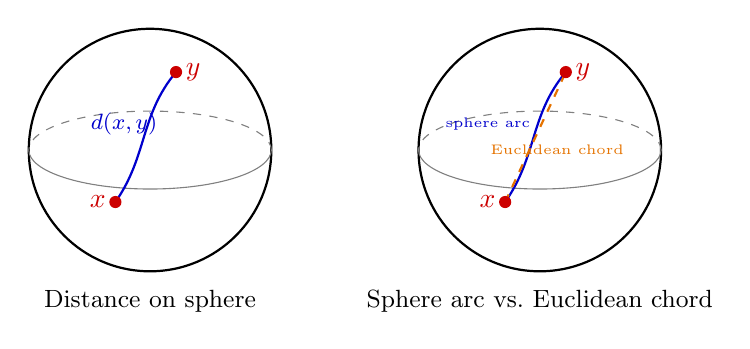
\begin{tikzpicture}[scale=1.1]
  \begin{scope}[shift={(0,0)}]
    \draw[thick] (0,0) circle (1.4);
    \draw[dashed, gray] (1.4,0) arc (0:180:1.4 and 0.45);
    \draw[gray] (-1.4,0) arc (180:360:1.4 and 0.45);
    \coordinate (x1) at (-0.4,-0.6);
    \coordinate (y1) at (0.3,0.9);
    \draw[blue!80!black, thick] (x1) to[out=55, in=230] (y1);
    \fill[red!80!black] (x1) circle (2pt) node[left] {$x$};
    \fill[red!80!black] (y1) circle (2pt) node[right] {$y$};
    \node[blue!80!black, font=\footnotesize] at (-0.3,0.3) {$d(x,y)$};
    \node[below, font=\small] at (0,-1.5) {Distance on sphere};
  \end{scope}

  \begin{scope}[shift={(4.5,0)}]
    \draw[thick] (0,0) circle (1.4);
    \draw[dashed, gray] (1.4,0) arc (0:180:1.4 and 0.45);
    \draw[gray] (-1.4,0) arc (180:360:1.4 and 0.45);
    \coordinate (x2) at (-0.4,-0.6);
    \coordinate (y2) at (0.3,0.9);
    \draw[blue!80!black, thick] (x2) to[out=55, in=230] (y2);
    \draw[orange!90!black, thick, dashed] (x2) -- (y2);
    \fill[red!80!black] (x2) circle (2pt) node[left] {$x$};
    \fill[red!80!black] (y2) circle (2pt) node[right] {$y$};
    \node[blue!80!black, font=\tiny] at (-0.6,0.3) {sphere arc};
    \node[orange!90!black, font=\tiny] at (0.2,0.0) {Euclidean chord};
    \node[below, font=\small] at (0,-1.5) {Sphere arc vs.\ Euclidean chord};
  \end{scope}
\end{tikzpicture}
\end{center}

\begin{exercise}[Supremum metric]
\label{ex:sup_metric_is_metric}
Show that the supremum metric from \cref{ex:metric_examples} \textbf{(c)} is a metric.
\end{exercise}

% Kept inline: solved directly in Corsin Nick/Class Notes/Week 2.pdf, p. 6.
\begin{exercisesolution}[Proof of \cref{ex:sup_metric_is_metric}]
Clearly, symmetry and definiteness hold. For the triangle inequality, let $f, g, h \in C^0([0,1])$ and
set $p := f - h$ and $q := h - g$. Then for all $x \in [0,1]$, we have:
\[|p(x)| \leq \sup|p| \qquad \text{and} \qquad |q(x)| \leq \sup|q|.\]
Adding the inequalities, we obtain for all $x \in [0,1]$:
\begin{align*}
|f(x) - g(x)| &= |p(x) + q(x)| \\
&\leq |p(x)| + |q(x)| \\
&\leq \sup|p| + \sup|q| \\
&= \sup|f - h| + \sup|h - g|.
\end{align*}
\end{exercisesolution}

% Quelle: Jérôme Paschoud/Notizen/Woche 2.1 Metrische Räume.pdf, p. 2
\begin{exercise}[$L^1$-metric]
\label{ex:integral_metric_is_metric}
Let $X := C^0([0,1], \mathbb{R})$ be the set of continuous functions $[0,1] \to \mathbb{R}$.
For $f,g \in X$, define
\[d(f,g) := \int_0^1 \lvert f(t)-g(t)\rvert\,dt.\]
Is $(X,d)$ a metric space? Provide a proof.
\end{exercise}

% Generator: Gemini 3.6 Pro
\begin{exercisesolution}[Proof of \cref{ex:integral_metric_is_metric}]
Yes, it is a metric space. We verify the three axioms of a metric:
\begin{enumerate}[label=\textbf{(\alph*)}]
  \item \textbf{Definiteness:} Clearly $d(f,g) \geq 0$ since the integrand $\lvert f(t)-g(t)\rvert$ is non-negative. If $f = g$, then $d(f,f) = \int_0^1 0\,dt = 0$. Conversely, suppose $d(f,g) = 0$. Since $\lvert f-g\rvert$ is a continuous, non-negative function, its integral over $[0,1]$ can only be zero if the integrand is identically zero. Thus $f(t) = g(t)$ for all $t \in [0,1]$, which means $f = g$.
  \item \textbf{Symmetry:} $d(f,g) = \int_0^1 \lvert f(t)-g(t)\rvert\,dt = \int_0^1 \lvert g(t)-f(t)\rvert\,dt = d(g,f)$.
  \item \textbf{Triangle inequality:} Let $f, g, h \in X$. The triangle inequality for real numbers yields $\lvert f(t)-h(t)\rvert \leq \lvert f(t)-g(t)\rvert + \lvert g(t)-h(t)\rvert$ for all $t \in [0,1]$. Integrating both sides, we obtain:
  \begin{align*}
  d(f,h) &= \int_0^1 \lvert f(t)-h(t)\rvert\,dt \\
  &\leq \int_0^1 \left(\lvert f(t)-g(t)\rvert + \lvert g(t)-h(t)\rvert\right)\,dt \\
  &= \int_0^1 \lvert f(t)-g(t)\rvert\,dt + \int_0^1 \lvert g(t)-h(t)\rvert\,dt \\
  &= d(f,g) + d(g,h).
  \end{align*}
\end{enumerate}
\end{exercisesolution}

% The old chapter closed here with a transition into "Open and closed sets"; that topic is now
% \cref{ch:open_closed}, whose own opening paragraph says the same thing, so the bridge is gone.

% --- exercises relocated here from the dissolved sheets ---

% Transition: Claude Opus 5 (Medium)
\begin{ainote}[Where the exercise-sheet problems live]
The official problem sheets are not reproduced as blocks anywhere in this document. Each problem
is quoted verbatim (from \texttt{exercises/ExN\_Analysis2\_eng.pdf}; attribution: Prof.\ Joaquim
Serra, D-MATH, ETH Z\"urich) and placed with the material it tests, so a problem from sheet 3 may
well appear several chapters away from a problem from sheet 2. Its solution is then in the
\emph{Solutions} section of that same chapter. Corsin's priority tags (\textbf{important},
\textbf{semi-important}, \textbf{optional}) and the official \textbf{(*)} difficulty marker are
carried along in each problem's title.
\end{ainote}

\begin{notation}
% Originally: content/exercise-sheets/week-02.tex, the sheet's own preamble.
Some problems in this document have a closed-answer format, similar to what you might find on the
final exam. \qt{Multiple Choice} means that zero, one or more answers can be correct. Questions
marked with (*) are a bit more complex, you might want to skip them at the first read.
\end{notation}

% Originally: content/week-02.tex, end of \section{Compactness}

\begin{aiexercise}[Equivalence of Manhattan and Supremum Metrics]
\label{ex:ai_metric_equivalence}
% Generator: Gemini 3.6 Flash (Medium)
Let $x := (x_1, x_2) \in \mathbb{R}^2$. Show that the Manhattan metric $d_1(x,0) := |x_1| + |x_2|$ and the supremum metric $d_3(x,0) := \max\{|x_1|, |x_2|\}$ satisfy the sharp inequalities:
\[
d_3(x,0) \leq d_1(x,0) \leq 2 \, d_3(x,0).
\]
\end{aiexercise}

% Originally: content/exercise-sheets/week-02.tex, problem 2.1
% Source: exercises/Ex2_Analysis2_eng.pdf, p. 1

\begin{exercise}[2.1 --- Examples and Non-examples of Metric spaces]
\label{ex:2.1}
Which of the following pairs are metric spaces? Prove it or provide a counterexample.
\begin{enumerate}[label=\textbf{\arabic*.}]
  \item $(B(X), d)$, where $B(X)$ denotes the set of all bounded functions from a non-empty set
    $X$ to $\mathbb{R}$ and
    $$d(f,g) := \sup_{x \in X} |f(x) - g(x)|.$$
  \item $(\mathbb{Q}_+, d)$, where $\mathbb{Q}_+$ are the positive rational numbers and
    $d(x,y) := \left|\tfrac{1}{x} - \tfrac{1}{y}\right|$.
  \item $(\mathbb{R}^2, d)$, where $d(x,y) := (x_1 - y_1)^2 + |x_2 - y_2|$.
  \item $(\mathbb{R}^2, d)$, where $d(x,y) := |x_1 - y_1|^{1/2} + |x_2 - y_2|$.
  \item $(\mathbb{R}^{n \times n}, d)$ with
    $d(X,Y) := \left(\Tr\{(X-Y)\transp(X-Y)\}\right)^{1/2}$.
  \item \textbf{(*)} $(\mathbb{R}^{n \times n}, d)$ with
    $$d(X,Y) := \sup\{|v\transp(X-Y)v| : v \in \mathbb{R}^n, \|v\| = 1\},$$
    and $\mathbb{R}^{n\times n}$ denoting the set of square matrices.
  \item \textbf{(*)} $(\mathbb{R}^2/\mathbb{Z}^2, d)$ where the flat 2-dimensional torus
    $\mathbb{R}^2/\mathbb{Z}^2$ is the set of equivalence classes of pairs of real numbers under
    the equivalence relation
    $$x, y \in \mathbb{R}^2, \quad x \sim y \iff x_1 - y_1 \in \mathbb{Z},\ x_2 - y_2 \in \mathbb{Z},$$
    and $d([x],[y]) := \inf_{k,h \in \mathbb{Z}} \|x - y + (k,h)\|$, with $\|\cdot\|$ denoting the
    Euclidean distance and $[x] \in \mathbb{R}^2/\mathbb{Z}^2$ denoting the equivalence class of
    $x \in \mathbb{R}^2$.
\end{enumerate}

\textit{Official hints:} \textbf{2.1.3} and \textbf{2.1.4} --- ignore what happens in the second
variable, it is there only to distract you. \textbf{2.1.5} --- rewrite, for a general matrix
$A := X - Y$, what $\Tr\{A\transp A\}^{1/2}$ actually means; it should look familiar.
\textbf{2.1.6} --- see what happens if $(X-Y)$ is anti-symmetric. \textbf{2.1.7} --- convince
yourself first that the ``inf'' is in fact a ``min''.
\end{exercise}

% Quelle: Diego Torres Tejeda/Notes - 02.03 - Diego Torres Tejeda.pdf, p. 2
\begin{ainote}[Diego's geometric intuition for the flat torus $\mathbb{R}^2/\mathbb{Z}^2$]
Diego's notes highlight the geometric picture behind part \textbf{2.1.7}: every equivalence class in $\mathbb{R}^2/\mathbb{Z}^2$ has a representative in $[0,1] \times [0,1]$. Identifying opposite boundaries $(0,x) \sim (1,x)$ and $(x,0) \sim (x,1)$ folds the unit square into a cylinder and subsequently into a 2D torus $\mathbb{T}^2 := \mathbb{R}^2/\mathbb{Z}^2$. The distance $d([x],[y])$ is simply the shortest Euclidean distance between points on this folded torus.
\end{ainote}

% Originally: content/exercise-sheets/week-02.tex, problem 2.5
% Source: exercises/Ex2_Analysis2_eng.pdf, p. 1

\begin{exercise}[2.5 --- Product of metric spaces]
\label{ex:2.5}
Let $(X, d_X)$ and $(Y, d_Y)$ be a pair of metric spaces. Recall that the set of ordered pairs
$(x,y)$ with $x \in X$ and $y \in Y$ is denoted by $X \times Y$. Consider the following functions
$X \times Y \to [0,\infty)$:
$$
\begin{aligned}
d_1((x,y),(x',y')) &:= \max\{d_X(x,x'), d_Y(y,y')\} \\
d_2((x,y),(x',y')) &:= d_X(x,x') + d_Y(y,y') \\
d_3((x,y),(x',y')) &:= \sqrt{d_X(x,x')^2 + d_Y(y,y')^2}.
\end{aligned}
$$
\begin{enumerate}[label=\textbf{\arabic*.}]
  \item Show that they are all valid distance functions on $X \times Y$.
  \item Show that they are all equivalent, i.e.\ there is a number $C > 0$ such that
    $$d_1((x,y),(x',y')) \leq C\,d_2((x,y),(x',y')) \leq C^2 d_3((x,y),(x',y')) \leq C^3 d_1((x,y),(x',y'))$$
    for all $x, x' \in X$, $y, y' \in Y$.
  \item Show that a sequence $(x_n, y_n) \to (x,y)$ with respect to $(X \times Y, d_3)$ if and
    only if $x_n \to x$ with respect to $d_X$ and $y_n \to y$ with respect to $d_Y$.
\end{enumerate}
\textit{Official hint:} don't get distracted by the abstract set-up --- you already know all
these things for $\mathbb{R} \times \mathbb{R}$; start from there, then rewrite those arguments in
this general framework.
\end{exercise}

% Originally: content/week-03.tex, \section{Cauchy--Schwarz} (Corsin Week 3, Friday)

\section{Cauchy--Schwarz}
\label{sec:cauchy_schwarz}

\subsection{Recap: inner products and norms}
\label{sec:inner_products_recap}

% Transition: Claude Opus 5 (High)
Corsin opens his Friday session by recalling the two definitions, which this chapter has already
stated in \cref{sec:structured_spaces}, where the hierarchy of structured spaces was drawn and
where the first supplements needed them. Rather than repeat them, here is what to have in mind:
\begin{itemize}
  \item An \emph{inner product} (\cref{def:inner_product}) is \textbf{bilinear},
    \textbf{symmetric} and \textbf{definite}. It measures length \emph{and} angle.
  \item A \emph{norm} (\cref{def:norm}) is \textbf{definite}, \textbf{homogeneous} and
    satisfies the \textbf{triangle inequality}. It measures length only.
  \item Each induces the next, via $\|v\| := \sqrt{\langle v,v\rangle}$ and
    $d(x,y) := \|x-y\|$, and neither implication reverses
    (\cref{prop:induced_norm_and_metric}, \cref{rem:norm_not_from_inner_product}).
\end{itemize}
What this section adds is the \emph{geometry}: why $\langle x,y\rangle$ deserves to be read as an
angle at all, and the resulting second proof of Cauchy--Schwarz.

\subsection{Geometric meaning of the inner product}

In $\mathbb{R}^2$, the following identity holds:
\[
\langle x,y\rangle := x_1y_1 + x_2y_2 = \|x\|\|y\|\cos\theta
\]
where $\theta$ is the angle between $x, y \in \mathbb{R}^2$.

To see this, conveniently choose our basis vectors such that $x = (x_1, 0)$, $y = (y_1, y_2)$.

\begin{center}
\begin{tikzpicture}[>=Latex, scale=1.1]
  \begin{scope}[shift={(0,0)}]
    \draw[->] (-0.3,0) -- (2.2,0);
    \draw[->] (0,-0.3) -- (0,2.2);
    \draw[blue!80!black, thick, ->] (0,0) -- (1.5,0.6) node[right] {$x$};
    \draw[orange!90!black, thick, ->] (0,0) -- (0.8,1.8) node[above] {$y$};
    \draw[purple, thick] (0.5,0.2) arc (21.8:66.0:0.5);
    \node[purple, font=\footnotesize] at (0.7,0.45) {$\theta$};
  \end{scope}

  \draw[->, thick] (2.4,1.0).. controls (2.8,1.3).. (3.3,1.0) node[midway, above, red, font=\tiny] {\shortstack{change of basis\\(rotation)}};

  % Same lengths and same angle as the left panel -- a rotation preserves both.
  % Left:  |x| = 1.616 at 21.80 deg, |y| = 1.970 at 66.04 deg, so theta = 44.24 deg.
  % Right: x rotated onto the axis at (1.616, 0), y at 44.24 deg with |y| unchanged.
  \begin{scope}[shift={(3.8,0)}]
    \draw[->] (-0.3,0) -- (2.5,0);
    \draw[->] (0,-0.3) -- (0,2.2);
    \draw[blue!80!black, thick, ->] (0,0) -- (1.616,0) node[below] {$x$};
    \draw[orange!90!black, thick, ->] (0,0) -- (1.411,1.375) node[above right] {$y$};
    \draw[dotted, gray] (1.411,1.375) -- (1.411,0);
    \draw[purple, thick] (0.5,0) arc (0:44.24:0.5);
    \node[purple, font=\footnotesize] at (0.72,0.22) {$\theta$};
  \end{scope}
\end{tikzpicture}
\end{center}

Then
\[
\langle x,y\rangle = x_1y_1 = x_1\|y\|\cos\theta = \|x\|\|y\|\cos\theta.
\]

For more rigour, you will show in Linalg that the rotations in $\mathbb{R}^2$ are given by
matrices $R$ satisfying $\langle Rx, Ry\rangle = \langle x,y\rangle$.

In a general inner product space $V$, this becomes the \textbf{definition} of the angle $\theta$.
It then makes sense to define the \newterm{projection onto $v$}, $\pi_v$:
\[
\pi_v(u) := \frac{\langle u,v\rangle}{\|v\|^2}\,v = \|u\|\cos\theta\,\frac{v}{\|v\|}.
\]

\begin{center}
\begin{tikzpicture}[>=Latex, scale=1.2]
  \draw[->] (-0.3,0) -- (3.5,0);
  \draw[->] (0,-0.3) -- (0,2.5);

  \draw[orange!90!black, thick, ->] (0,0) -- (3.2,0.8) node[right] {$v$};
  \draw[blue!80!black, thick, ->] (0,0) -- (1.2,2.0) node[above left] {$u$};

  \coordinate (P) at (1.60, 0.40);
  \coordinate (U) at (1.2, 2.0);

  \draw[purple!80!black, thick, dashed] (U) -- (P);
  \fill[purple!80!black] (P) circle (2pt) node[below right, font=\small] {$\pi_v(u)$};

  \draw[green!60!black, thick] (0.5,0.125) arc (14:59:0.5);
  \node[green!60!black, font=\small] at (0.6,0.3) {$\theta$};
\end{tikzpicture}
\end{center}

In words, $\pi_v(u)$ is the part of $u$ which points along $v$. In particular,
\[
\|\pi_v(u)\| = \|u\|\,|\cos\theta| = \frac{|\langle u,v\rangle|}{\|v\|}.
\]
In this sense, Cauchy--Schwarz says something visually obvious. Reading the picture above, all
three of the following are the same statement:
\[
\frac{|\langle u,v\rangle|}{\|v\|} \leq \|u\| \iff \|\pi_v(u)\| \leq \|u\| \iff \|u\|\,|\cos\theta| \leq \|u\|.
\]

\begin{remark}[Hint for the proof of Cauchy--Schwarz]
\label{rem:proof_hint_cauchy_schwarz}
Use definiteness and expand the term
\[
\langle u - \pi_v(u),\ u - \pi_v(u)\rangle = \dots
\]
where $u - \pi_v(u)$ is the \textbf{perpendicular part} of $u$ to $v$.
\end{remark}

% Sonnet 5 (Medium)
\subsection{The Cauchy--Schwarz inequality}

% Corsin's own notes stop at the hint above (rem:proof_hint_cauchy_schwarz) and never state the
% inequality itself as a formal result, which is notable given that it names the section. The
% theorem below fills that in, carrying out exactly the computation he hints at.

\begin{theorem}[Cauchy--Schwarz inequality]
\label{thm:cauchy_schwarz}
Let $V$ be an inner product space (\cref{def:inner_product}) with induced norm
$\|\cdot\| := \sqrt{\langle\cdot,\cdot\rangle}$ (\cref{def:norm}). Then for all $u,v \in V$,
\[|\langle u,v\rangle| \leq \|u\|\,\|v\|,\]
with equality if and only if $u,v$ are linearly dependent.
\end{theorem}

\begin{proof}
If $v = 0$, both sides vanish and the claim holds trivially, so assume $v \neq 0$. Following
\Cref{rem:proof_hint_cauchy_schwarz}, definiteness (\cref{def:inner_product}) gives
\[
  0 \ \leq\ \langle u-\pi_v(u),\ u-\pi_v(u)\rangle
    \ =\ \langle u,u\rangle - 2\langle u,\pi_v(u)\rangle + \langle \pi_v(u),\pi_v(u)\rangle.
\]
Using $\pi_v(u) = \tfrac{\langle u,v\rangle}{\|v\|^2}v$ and bilinearity, the two right-hand terms
are
\begin{align*}
  \langle u,\pi_v(u)\rangle &= \frac{\langle u,v\rangle^2}{\|v\|^2}, \\[0.3ex]
  \langle \pi_v(u),\pi_v(u)\rangle
    &= \frac{\langle u,v\rangle^2}{\|v\|^4}\langle v,v\rangle
     = \frac{\langle u,v\rangle^2}{\|v\|^2}.
\end{align*}
Note that the two are equal, so substituting them leaves a single copy behind:
\[
  0 \ \leq\ \|u\|^2 - \frac{2\langle u,v\rangle^2}{\|v\|^2} + \frac{\langle u,v\rangle^2}{\|v\|^2}
    \ =\ \|u\|^2 - \frac{\langle u,v\rangle^2}{\|v\|^2}.
\]
This rearranges to $\langle u,v\rangle^2 \leq \|u\|^2\|v\|^2$, that is,
$|\langle u,v\rangle| \leq \|u\|\,\|v\|$. By definiteness, equality holds if and only if
$u - \pi_v(u) = 0$, which says precisely that $u$ is a scalar multiple of $v$.
\end{proof}

% Generator: Claude Opus 5 (High)
\begin{remark}[The same proof twice]
\label{rem:two_proofs_cauchy_schwarz}
This is the second proof of Cauchy--Schwarz in these notes;
\cref{prop:cauchy_schwarz_geometric_proof} gave another, following Diego Torres
Tejeda. The two look different at first. One minimises the quadratic
$f(\lambda) := \|v-\lambda w\|^2$ over $\lambda$, while the other expands
$\|u-\pi_v(u)\|^2 \geq 0$. But the minimiser found in the first is
$\lambda_0 = \tfrac{\langle v,w\rangle}{\|w\|^2}$, which is exactly the coefficient defining
$\pi_w(v)$. Consequently, the first proof \emph{derives} the projection by optimisation, and the
second \emph{postulates} it and checks that it works. Keeping both is worthwhile precisely because
the pair shows where the projection comes from. It is not a lucky guess, but the closest point of
the line to $v$.
\end{remark}


% --- exercises relocated here from the dissolved sheets ---

% Originally: content/exercise-sheets/week-03.tex, problem 3.7
% Source: exercises/Ex3_Analysis2_eng.pdf

\begin{exercise}[3.7 --- Cauchy--Schwarz]
\label{ex:3.7}
Let $V$ be a vector space over $\mathbb{R}$, let $\langle\cdot,\cdot\rangle$ be an inner product
on $V$, and let $\|\cdot\| : V \to \mathbb{R}$ be given by $\|v\| = \sqrt{\langle v,v\rangle}$.
Then the inequality
\begin{equation*}
|\langle v,w\rangle| \leq \|v\|\|w\| \tag{1}
\end{equation*}
holds for all $v, w \in V$. Furthermore, equality in (1) holds if and only if $v$ and $w$ are
linearly dependent.
\end{exercise}

\begin{remark}
Corsin devotes the whole second half of Friday (\cref{sec:cauchy_schwarz}) to this problem,
including the geometric reading and an explicit proof hint.
\end{remark}

% Originally: content/exercise-sheets/week-03.tex, problem 3.8
% Source: exercises/Ex3_Analysis2_eng.pdf

\begin{exercise}[3.8 --- Inner product and norm]
\label{ex:3.8}
Let $V$ be a vector space over $\mathbb{R}$, let $\langle -,-\rangle$ be an inner product on $V$.
The map defined by
$$\|\cdot\| : V \to \mathbb{R}, \qquad \|v\| = \sqrt{\langle v,v\rangle}$$
satisfies the triangular inequality and is a norm.
\end{exercise}

% Originally: content/exercise-sheets/week-03.tex, problem 3.9
% Source: exercises/Ex3_Analysis2_eng.pdf

\begin{exercise}[3.9 --- All norms are equivalent in $\mathbb{R}^n$]
\label{ex:3.9}
Let $|\cdot|$ denote the standard Euclidean norm in $\mathbb{R}^n$ and let
$f : \mathbb{R}^n \to [0,\infty)$ be another norm (that is, a function satisfying the properties
of \textit{Definition 9.89}).
\begin{enumerate}[label=\textbf{\arabic*.}]
  \item Expressing $x$ in a basis and using the ``abstract'' properties that $f$ must have, show
    that there is a constant $C_1 > 0$ such that $f(x) \leq C_1|x|$ for all $x \in \mathbb{R}^n$.
  \item Show that $f$ is continuous in $\mathbb{R}^n$ (with respect to the standard distance of
    $\mathbb{R}^n$!).
  \item Show that there is a number $c_2 > 0$ such that $f(x) \geq c_2$ for all $|x| = 1$.
  \item Conclude that $f(x) \geq c_2|x|$ for all $x \in \mathbb{R}^n$.
  \item Show that if $\tilde f$ is yet another norm, then there is $C > 0$ such that
    $C^{-1}f(x) \leq \tilde f(x) \leq Cf(x)$ for all $x \in \mathbb{R}^n$.
\end{enumerate}
\exhint[Official hints]{\textbf{3.9.2:} recall that from the definition it follows that
$|f(x) - f(y)| \leq f(x-y)$, and that Lipschitz functions are always continuous.
\textbf{3.9.3:} apply the Weierstrass theorem to $f$ on $S := \{x \in \mathbb{R}^n : |x| = 1\}$
and use that $f$, being a norm, is nondegenerate. \textbf{3.9.5:} if $f$ is equivalent to $|\cdot|$ and
$\tilde f$ is equivalent to $|\cdot|$, it follows by transitivity that $f$ is equivalent to
$\tilde f$.}
\end{exercise}

\begin{remark}
Hint 3.9.3 is exactly Corsin's reason \#2 for caring about compactness
(\cref{sec:why_compactness_matters}), namely the Weierstrass extreme value theorem applied on the
compact unit sphere.
\end{remark}

% Supplement: Analysis_II_Script_v1.pdf, p. 35
\begin{exercise}[The polynomial ring $\mathbb{R}{[}x{]}$ is infinite-dimensional]
\label{ex:polynomials_infinite_dimensional}
Show that the vector space $\mathbb{R}[x]$ of polynomials with real coefficients is infinite
dimensional, and exhibit a basis.
\end{exercise}

\begin{remark}
This is exactly the hypothesis \cref{ex:3.9} needs and cannot do without.
\Cref{rem:norm_equivalence_needs_finite_dimension} already gave $C^0([0,1],\mathbb{R})$ as an
infinite-dimensional space where norm equivalence fails. Note that $\mathbb{R}[x]$ is the
algebraically simplest such example, with an explicit basis and no analysis required at all.
\end{remark}

% Originally: content/exercise-sheets/week-03.tex, problem 3.10
% Source: exercises/Ex3_Analysis2_eng.pdf

\begin{exercise}[3.10 --- Hilbert--Schmidt norm of the composition]
\label{ex:3.10}
Take two linear functions $\varphi : \mathbb{R}^d \to \mathbb{R}^n$ and
$\psi : \mathbb{R}^n \to \mathbb{R}^m$, and denote with $\Phi$, $\Psi$ the matrices that represent
them in the canonical bases. Recall that the linear map
$\psi \circ \varphi : \mathbb{R}^d \to \mathbb{R}^m$ is represented in these bases by the matrix
$\Psi \cdot \Phi$. Show that
$$\|\Psi \cdot \Phi\| \leq \|\Psi\|\|\Phi\|,$$
where $\|\cdot\|$ is the Hilbert--Schmidt norm of a matrix (see \textit{Definition 9.96} in the
notes).

\exhint[Official hint]{Recall that $\|M\|^2$ is the sum of the squares of the entries of $M$.
Notice that $(\Psi\cdot\Phi)^i_j$ ($i$-th row, $j$-th column) is the scalar product of $\Psi^i$
and $\Phi_j$, which are vectors of $\mathbb{R}^n$. Apply Cauchy--Schwarz to each of them.}
\end{exercise}

% Originally: content/week-04.tex, \exercisesheet{4}
% Source: exercises/Ex4_Analysis2_eng.pdf

\begin{exercise}[4.3 --- $p$-norms \textnormal{(semi-important; parts 4 and 6 important)}]
\label{ex:4.3}
For $p \geq 1$ and $x \in \mathbb{R}^n$ define the \textbf{$p$-norm} of $x$ as
\[|x|_p := \Big(\sum_{i=1}^{n} |x_i|^p\Big)^{1/p}.\]
\begin{enumerate}[label=\textbf{\arabic*.}]
  \item For $n = 2$ and $p = 1, 2, 10$ sketch the sets $\{x \in \mathbb{R}^2 : |x|_p \leq 1\}$.
  \item For a given $x \in \mathbb{R}^n$, compute the limit
    $|x|_\infty := \lim_{p\to\infty}|x|_p$.
  \item Using an appropriate inequality that you have seen in class, prove that
    \[\Big(\sum_{i=1}^{n} a_i^{p-1}b_i\Big)^2 \leq \Big(\sum_{i=1}^{n}a_i^p\Big)\Big(\sum_{i=1}^{n}a_i^{p-2}b_i^2\Big),\]
    whenever $a_i, b_i$ are $n$-tuples of positive numbers.
  \item Fix $x, y \in \mathbb{R}^n$ and consider the function $f : [0,1] \to \mathbb{R}$ defined
    as
    \begin{equation*}
    f(t) := |tx + (1-t)y|_p = \Big(\sum_{i=1}^{n}|tx_i + (1-t)y_i|^p\Big)^{1/p}. \tag{1}
    \end{equation*}
    Show that $f$ is convex. You may assume that the coordinates of $x$ and $y$ are all strictly
    positive and use the inequality of the previous point.
  \item Deduce from the previous point that the triangular inequality holds, i.e.\
    $|x+y|_p \leq |x|_p + |y|_p$ for all $x,y \in \mathbb{R}^n$.
  \item What happens for $p \in (0,1)$?
\end{enumerate}
\exhint[Official hints]{\textbf{4.3.3:} use Cauchy--Schwarz and the fact that
$a_i^{p-1}b_i = a_i^{p/2}\cdot a_i^{(p-2)/2}b_i$. \textbf{4.3.4:} show that $f''(t) \geq 0$; it
is not the simplest derivative, but if you get it right the inequality in 4.3.3 will be just what
you need. \textbf{4.3.5:} write the convexity inequality between $x$, $y$ and the middle point
$(x+y)/2$. To get the general case from the one with positive coordinates, observe that for
$x \in \mathbb{R}^n$, denoting $\hat x := (|x_1|,\dots,|x_n|)$, we have
$|x+y|_p \leq |\hat x + \hat y|_p$ and $|\hat x|_p = |x|_p$ for all $x,y \in \mathbb{R}^n$.}
\end{exercise}

% Originally: content/exercise-sheets/week-04.tex, problem 4.4 --- never previously built
% Source: exercises/Ex4_Analysis2_eng.pdf

\begin{exercise}[4.4 --- $p$-means \textnormal{(optional)}]
\label{ex:4.4}
For $x \in \mathbb{R}^n$ with positive coordinates and $p \neq 0$ define the \textbf{$p$-mean} as
$$\mu_p(x) := \left(\frac{x_1^p + \dots + x_n^p}{n}\right)^{1/p}.$$
\begin{enumerate}[label=\textbf{\arabic*.}]
  \item Compute the limits $p \to \pm\infty$, $p \to 0$ and define accordingly
    $\mu_{-\infty}(x)$, $\mu_0(x)$, $\mu_{+\infty}(x)$.
  \item For any $n$-tuple of numbers $a_i > 0$ show that
    $$\sum_{i=1}^{n} \frac{a_i\log(a_i)}{a_1 + \dots + a_n} \geq \log\left(\frac{a_1 \dots + a_n}{n}\right).$$
  \item For a fixed $x$, show that the function $f : \mathbb{R}\to\mathbb{R}$, given by
    $f(t) := \mu_t(x)$, is continuous and increasing.
  \item Prove the Arithmetic--Geometric inequality and Arithmetic--Quadratic inequality:
    $$n(x_1x_2\cdots x_n)^{1/n} \leq x_1 + \dots + x_n, \qquad (x_1+\dots+x_n)^2 \leq n(x_1^2+\dots+x_n^2).$$
  \item \textbf{(*)} Is $f$ continuously differentiable in the whole $\mathbb{R}$?
\end{enumerate}
\exhint[Official hints]{\textbf{4.4.2:} combine the concavity of $\log(\cdot)$ and the
Cauchy--Schwarz inequality; use the generalisation of the concavity inequality: for any concave
$f : \mathbb{R}\to\mathbb{R}$,
$f(\lambda_1x_1 + \dots + \lambda_nx_n) \geq \lambda_1f(x_1)+\dots+\lambda_nf(x_n)$ for all
$x_i \in \mathbb{R}$, $0 \leq \lambda_i \leq 1$ with $\lambda_1+\dots+\lambda_n = 1$.
\textbf{4.4.3:} it might be more convenient to work with $\log f(t)$.}
\end{exercise}

% Originally: new section, 2026-08-09. Not a move --- this material had no home in the document
% before. Exercise 3.9 asked the reader to prove that all norms on R^n are equivalent, and the
% solution in 99-solutions.tex proved it, but the statement itself was nowhere in the body, so
% nothing could \cref it and the reader met the result only as homework.
% Supplement: lec_notes.pdf, pp. 31--33 (Definition 9.105, Theorem 9.107, Corollary 9.109)
% Generator: Claude Opus 5 (High)

\section{Equivalence of norms}
\label{sec:equivalence_of_norms}

The previous sections put several norms on the same vector space: the Euclidean norm, the
$p$-norms, the supremum norm. A natural worry follows. Convergence, openness, continuity and
compactness were all defined from a metric, and on a normed space that metric came from the norm.
So does changing the norm change which sequences converge and which sets are open?

On $\mathbb{R}^n$ the answer is no, and the reason is worth isolating, because it is one of the
few places in this course where finite-dimensionality is doing essential work.

% Supplement: lec_notes.pdf, p. 31 (Definition 9.105)
\begin{definition}[Equivalent norms]
\label{def:equivalent_norms}
Let $V$ be a vector space over $\mathbb{R}$ and let $\|\cdot\|_1$ and $\|\cdot\|_2$ be two norms
on $V$. They are called \newterm{equivalent} \germanfor{äquivalent}, or \emph{comparable}, if
there are constants $A, B > 0$ with
\[\|v\|_1 \leq A\|v\|_2 \qquad\text{and}\qquad \|v\|_2 \leq B\|v\|_1 \qquad\text{for all } v \in V.\]
\end{definition}

\begin{remark}[Why two inequalities and not one]
A single inequality $\|v\|_1 \leq A\|v\|_2$ says only that $\|\cdot\|_2$-convergence implies
$\|\cdot\|_1$-convergence: it makes the first norm the coarser of the two. Equivalence is the
two-sided statement, and it is exactly what is needed for the two norms to have the same null
sequences, and hence the same convergent sequences, open sets and compact sets. That equivalence
of norms really is an equivalence relation is part 5 of \cref{ex:3.9}.
\end{remark}

% Supplement: lec_notes.pdf, p. 32 (Example 9.106)
\begin{example}[The $1$-norm against the maximum norm]
\label{ex:one_norm_vs_max_norm}
On $\mathbb{R}^n$,
\[\|v\|_\infty \leq \|v\|_1 \qquad\text{and}\qquad \|v\|_1 \leq n\|v\|_\infty,\]
so the two are equivalent with $A = 1$ and $B = n$. The left inequality holds because the largest
$|v_i|$ is one of the terms of the sum $\sum_i|v_i|$; the right because each of the $n$ terms of
that sum is at most $\max_i|v_i|$.

The constant $n$ on the right is sharp, as $v = (1,1,\dots,1)$ shows, and it is the first sign of
what goes wrong later: the constants in \cref{thm:all_norms_equivalent} are allowed to depend on
the dimension, and there is no dimension to depend on in an infinite-dimensional space.
\end{example}

% Supplement: lec_notes.pdf, p. 32 (Theorem 9.107)
\begin{theorem}[All norms on $\mathbb{R}^n$ are equivalent]
\label{thm:all_norms_equivalent}
Any two norms on $\mathbb{R}^n$ are equivalent in the sense of \cref{def:equivalent_norms}.
\end{theorem}

\begin{proof}
This is \cref{ex:3.9}, whose five parts are exactly the five steps of the argument, and it is
proved in full in the solutions to that exercise. In outline, with $|\cdot|$ the Euclidean norm
and $f$ an arbitrary norm: expanding $x$ in the standard basis and applying the triangle
inequality, homogeneity and Cauchy--Schwarz gives $f(x) \leq C_1|x|$; that bound makes $f$
Lipschitz, hence continuous, for the Euclidean metric; Weierstrass then gives $f$ a positive
minimum $c_2$ on the Euclidean unit sphere, which is compact by Heine--Borel
(\cref{thm:heine_borel}); and homogeneity spreads that bound from the sphere to all of
$\mathbb{R}^n$, giving $f(x) \geq c_2|x|$.
\end{proof}

\begin{remark}[Where each hypothesis is used]
\label{rem:where_finite_dimension_enters}
Both halves of the proof use finite-dimensionality, and they use it differently. The first
inequality expands $x$ in a \emph{finite} basis, so the sum of $n$ terms it produces is a sum and
not a series. The second applies Weierstrass on the unit sphere, which needs that sphere to be
\emph{compact}, and by Heine--Borel it is, in $\mathbb{R}^n$ and nowhere else.
\Cref{rem:norm_equivalence_needs_finite_dimension} exhibits the failure in
$C^0([0,1],\mathbb{R})$, and \cref{ex:polynomials_infinite_dimensional} gives the algebraically
simplest infinite-dimensional space to have in mind.
\end{remark}

% Supplement: lec_notes.pdf, p. 33 (9.108)
\begin{corollary}[Any finite-dimensional real vector space]
\label{cor:all_norms_equivalent_finite_dim}
Let $V$ be a real vector space of finite dimension $n$. Then any two norms on $V$ are equivalent.
\end{corollary}

\begin{proof}
Fix a basis $\mathcal{B} = \{e_1,\dots,e_n\}$ of $V$. The coordinate map
$\iota_{\mathcal{B}} : \mathbb{R}^n \to V$, $(x_1,\dots,x_n) \mapsto x_1e_1+\dots+x_ne_n$, is a
linear isomorphism, so a norm $\|\cdot\|$ on $V$ pulls back to the norm
$x \mapsto \|\iota_{\mathcal{B}}(x)\|$ on $\mathbb{R}^n$, and the two-sided inequalities of
\cref{def:equivalent_norms} are preserved in both directions under this identification. Applying
\cref{thm:all_norms_equivalent} on $\mathbb{R}^n$ and transporting back gives the claim.
\end{proof}

% Supplement: lec_notes.pdf, p. 33 (Corollary 9.109)
\begin{corollary}[All norms give the same topology]
\label{cor:norms_same_topology}
Topological properties of a subset $E \subseteq \mathbb{R}^n$ (openness, closedness, convergence
of sequences, compactness, connectedness) do not depend on which norm was used to define the
metric.
\end{corollary}

\begin{proof}
Let $d_1, d_2$ be the metrics induced by two norms. By \cref{thm:all_norms_equivalent} there is a
constant $C > 0$ with $C^{-1}d_1(x,y) \leq d_2(x,y) \leq Cd_1(x,y)$ for all $x,y$, since
$d_i(x,y) = \|x-y\|_i$ and the norms are equivalent. Hence every $d_1$-ball contains a
$d_2$-ball about the same centre and conversely, which by \cref{def:open_closed} makes a set open
for $d_1$ exactly when it is open for $d_2$. The two metrics therefore generate the same
topology, and every property defined purely in terms of the open sets agrees.
\end{proof}

\begin{ainote}[What this licenses, and what it does not]
\label{ainote:norm_equivalence_scope}
\Cref{cor:norms_same_topology} is the reason this document is free to say \qt{open}, \qt{compact}
or \qt{convergent} in $\mathbb{R}^n$ without ever naming a norm, and it is worth knowing that the
licence has been earned rather than assumed.

Three things it does \emph{not} give you.
\begin{itemize}
  \item It is about \emph{topological} properties only. Metric quantities are not preserved:
    the unit ball genuinely changes shape with the norm (see the three drawn in
    \cref{sec:unit_balls}), distances change, and so do Lipschitz constants. A $1$-Lipschitz map
    for one norm need not be $1$-Lipschitz for another, only Lipschitz with some other constant.
  \item It says nothing in infinite dimensions, where the conclusion is false
    (\cref{rem:where_finite_dimension_enters}).
  \item It does not make the choice of norm irrelevant in practice. Estimates are still written
    in whichever norm makes the constants come out cleanly, which is why the supremum norm is the
    one used on $C(K,\mathbb{R}^m)$ in \cref{sec:ascoli_arzela} even though that space is
    infinite-dimensional and the theorem above does not reach it.
\end{itemize}
\end{ainote}

% Originally: the \section{Solutions} of content/week-02.tex and content/week-03.tex

\section{Solutions}
\label{sec:metric_spaces_solutions}

\begin{ainote}[How the solutions in this document were produced]
Where a tutor solves a problem in their own notes, that solution is kept \emph{inline}, directly
after the statement, mirroring how they present it --- each such case carries a
\texttt{\% Kept inline} comment naming the source page. Everything else is collected in a
\emph{Solutions} section like this one at the end of the chapter that hosts the problem. Those
were worked independently and only then checked against the official
\texttt{exercises/SolN\_Analysis2\_eng.pdf}; wherever the comparison turned up anything worth
flagging, it is flagged in an AI-Note next to the solution.
\end{ainote}

\begin{exercisesolution}[Proof of \cref{ex:ai_metric_equivalence}]
% Generator: Gemini 3.6 Flash (Medium)
For any $x = (x_1, x_2) \in \mathbb{R}^2$, we have $\max\{|x_1|, |x_2|\} \leq |x_1| + |x_2|$, giving $d_3(x,0) \leq d_1(x,0)$. Conversely, since $|x_1| \leq \max\{|x_1|, |x_2|\}$ and $|x_2| \leq \max\{|x_1|, |x_2|\}$, summing these yields $|x_1| + |x_2| \leq 2 \max\{|x_1|, |x_2|\}$, i.e., $d_1(x,0) \leq 2 \, d_3(x,0)$. Both bounds are sharp: equality on the left holds for $x=(1,0)$, and equality on the right holds for $x=(1,1)$.
\end{exercisesolution}

\begin{exercisesolution}[Solution to \cref{ex:2.1}]
% Generator: Claude Opus 5 (High)
Throughout, non-negativity and symmetry are immediate in every part and are not belaboured; the
interest is in \textbf{definiteness} and the \textbf{triangle inequality}.
\begin{enumerate}[label=\textbf{\arabic*.}]
  \item \textbf{Yes.} Boundedness of $f$ and $g$ makes the supremum finite, so $d$ really maps
    into $\mathbb{R}$. Definiteness: $d(f,g)=0$ forces $|f(x)-g(x)| = 0$ for every $x$, i.e.\
    $f=g$. For the triangle inequality, estimate pointwise and only then take the supremum:
    \[|f(x)-h(x)| \leq |f(x)-g(x)| + |g(x)-h(x)| \leq d(f,g) + d(g,h) \quad \text{for all } x,\]
    so the right-hand side is an upper bound for $|f-h|$ and hence dominates $d(f,h)$. This is
    \cref{ex:sup_metric_is_metric} verbatim, with $[0,1]$ replaced by an arbitrary set $X$ and
    continuity replaced by boundedness --- note that it was boundedness, not continuity, that
    the argument there actually used.
  \item \textbf{Yes.} Let $\varphi(x) := 1/x$, an injective map $\mathbb{Q}_+ \to \mathbb{Q}_+$,
    and observe that $d(x,y) = |\varphi(x)-\varphi(y)|$. Symmetry and the triangle inequality
    are inherited from $|\cdot|$ without any work, and definiteness is exactly injectivity of
    $\varphi$: from $d(x,y)=0$ we get $1/x = 1/y$, hence $x=y$. This is the same pullback
    construction as \cref{ex:completeness_not_topological}, and the same warning applies ---
    pulling a metric back along an injection \emph{always} produces a metric, which is why the
    interesting question about such a $d$ is never whether it is one, but whether it is
    complete.
  \item \textbf{No} --- the triangle inequality fails. Ignore the second coordinate, as the
    official hint suggests, and take three collinear points $x := (0,0)$, $y := (1,0)$ and
    $z := (2,0)$:
    \[d(x,z) = 2^2 = 4 \quad > \quad d(x,y) + d(y,z) = 1 + 1 = 2.\]
    Squaring produces the same failure as in
    \cref{ex:metric_axioms_are_needed}\textbf{(c)}: a function growing faster than linearly
    makes one long step more expensive than two short ones.
  \item \textbf{Yes.} A sum of two metrics acting on separate coordinates is a metric, so
    everything reduces to the first coordinate, where the claim is that
    $(s,t) \mapsto |s-t|^{1/2}$ satisfies the triangle inequality on $\mathbb{R}$. That follows
    from \textbf{subadditivity of the square root}, $\sqrt{a+b} \leq \sqrt a + \sqrt b$ for
    $a,b \geq 0$, which holds because squaring the right-hand side gives
    $a+b+2\sqrt{ab} \geq a+b$. Hence
    \[|x_1-z_1|^{1/2} \leq \big(|x_1-y_1| + |y_1-z_1|\big)^{1/2}
      \leq |x_1-y_1|^{1/2} + |y_1-z_1|^{1/2}.\]
    Contrast this with part 3: $\sqrt{\cdot}$ is concave and vanishes at $0$, hence subadditive,
    while $(\cdot)^2$ is convex, hence super-additive. That single distinction settles both
    parts.
  \item \textbf{Yes.} Write $A := X-Y$. Then
    \[\Tr(A\transp A) = \sum_{i=1}^n (A\transp A)_{ii} = \sum_{i,j=1}^n A_{ji}^2,\]
    so $d(X,Y)$ is nothing but the Euclidean distance between $X$ and $Y$ regarded as vectors of
    $\mathbb{R}^{n^2}$, and it is a metric by
    \cref{prop:induced_norm_and_metric}\textbf{(b)}. The associated norm is the
    \newterm{Frobenius norm} (\germanterm{Frobeniusnorm}), also called the Hilbert--Schmidt norm.
  \item \textbf{No} --- and here it is \textbf{definiteness} that fails, not the triangle
    inequality. Following the hint, suppose $A := X-Y$ is \emph{anti-symmetric},
    $A\transp = -A$. For any $v$ the number $v\transp Av$ is a $1\times1$ matrix, hence equal to
    its own transpose:
    \[v\transp A v = (v\transp A v)\transp = v\transp A\transp v = -\,v\transp A v,\]
    so $v\transp Av = 0$ for \emph{every} $v$. Taking $n=2$ with
    \[X := \begin{pmatrix} 0 & 1 \\ -1 & 0\end{pmatrix}, \qquad
      Y := \begin{pmatrix} 0 & 0 \\ 0 & 0\end{pmatrix}\]
    gives $X \neq Y$ but $d(X,Y) = 0$. Every other axiom does hold, so $d$ is a
    \newterm{pseudo-metric} (\germanterm{Pseudometrik}): it cannot separate two matrices
    differing by an anti-symmetric one. Equivalently, it restricts to a genuine metric on the
    symmetric matrices.
  \item \textbf{Yes.} Three things need checking, and the first is the one that is easy to skip.

    \textit{Well defined.} Replacing $x$ by $x+(m,n)$ and $y$ by $y+(m',n')$ shifts $x-y$ by the
    integer vector $(m-m',\,n-n')$, which merely re-indexes the infimum. So $d([x],[y])$ does
    not depend on the representatives chosen.

    \textit{The infimum is a minimum.} Only finitely many integer vectors $(k,h)$ satisfy
    $\lVert x-y+(k,h)\rVert \leq \lVert x-y\rVert$, because $\mathbb{Z}^2$ is discrete; the
    infimum is therefore taken over a finite non-empty set of candidates and is attained. This
    is what the official hint asks you to settle first, and it is what makes the next step
    legitimate.

    \textit{Definiteness.} If $d([x],[y]) = 0$ then, the minimum being attained,
    $x-y+(k,h) = 0$ for some integers $k,h$, that is $x \sim y$ and $[x] = [y]$. Note exactly
    where \qt{the infimum is a minimum} was needed: an infimum equal to $0$ but not attained
    would say nothing at all.

    \textit{Triangle inequality.} Choose minimisers $(k_1,h_1)$ for the pair $(x,y)$ and
    $(k_2,h_2)$ for $(y,z)$. Their sum is a legitimate candidate for the pair $(x,z)$, so
    \begin{align*}
      d([x],[z]) &\leq \big\lVert x-z+(k_1{+}k_2,\ h_1{+}h_2)\big\rVert \\
      &= \big\lVert \big(x-y+(k_1,h_1)\big) + \big(y-z+(k_2,h_2)\big)\big\rVert \\
      &\leq d([x],[y]) + d([y],[z]).
    \end{align*}
\end{enumerate}
\end{exercisesolution}

\begin{ainote}
Parts 3, 4 and 6 are the ones worth revisiting, because each breaks (or rescues) a different
axiom and together they cover every way the definition can fail. Part 3 kills the triangle
inequality by growing too fast; part 4 rescues it by growing slowly enough; part 6 satisfies the
triangle inequality perfectly and fails on definiteness instead. Read alongside
\cref{ex:metric_axioms_are_needed}, they make the case that the three axioms are genuinely
independent.
\end{ainote}

\begin{exercisesolution}[Solution to \cref{ex:2.5}]
% Generator: Claude Opus 5 (High)
Write $s := d_X(x,x')$ and $t := d_Y(y,y')$ throughout, so that the three candidates are
$d_1 = \max\{s,t\}$, $d_2 = s+t$ and $d_3 = \sqrt{s^2+t^2}$ --- that is, the supremum, Manhattan
and standard metrics of \cref{ex:metric_examples} applied to the pair $(s,t)$. Almost everything
below is that one observation.
\begin{enumerate}[label=\textbf{\arabic*.}]
  \item \textbf{All three are metrics.} Each vanishes exactly when $s = t = 0$, i.e.\ when
    $x=x'$ and $y=y'$, which is definiteness; symmetry is inherited from $d_X$ and $d_Y$. For
    the triangle inequality, set
    \[a := \big(d_X(x,x'),\,d_Y(y,y')\big), \quad
      b := \big(d_X(x',x''),\,d_Y(y',y'')\big), \quad
      c := \big(d_X(x,x''),\,d_Y(y,y'')\big),\]
    all lying in $[0,\infty)^2$. The triangle inequalities in $X$ and in $Y$ say precisely that
    $c \leq a+b$ \emph{componentwise}. Each of $\max$, the sum and $\lVert\cdot\rVert_2$ is
    monotone on $[0,\infty)^2$ and subadditive, so
    \[N(c) \ \leq\ N(a+b) \ \leq\ N(a) + N(b)\]
    for $N \in \{\max,\ \textstyle\sum,\ \lVert\cdot\rVert_2\}$ --- which is the required
    inequality in all three cases at once.
  \item \textbf{Equivalence.} For all $s,t \geq 0$,
    \[\max\{s,t\} \ \leq\ \sqrt{s^2+t^2} \ \leq\ s+t \ \leq\ 2\max\{s,t\},\]
    i.e.\ $d_1 \leq d_3 \leq d_2 \leq 2d_1$; the middle inequality holds because
    $(s+t)^2 = s^2+t^2+2st \geq s^2+t^2$. Hence $C := 2$ satisfies the chain in the statement:
    $d_1 \leq 2d_2$, then $2d_2 \leq 4d_3$ (since $d_2 \leq \sqrt2\,d_3$ by Cauchy--Schwarz,
    and $\sqrt2 \leq 2$), and finally $4d_3 \leq 8d_1$ (since $d_3 \leq \sqrt2\,d_1$).
  \item \textbf{Convergence is coordinatewise.} From part 2,
    \[\max\big\{d_X(x_n,x),\ d_Y(y_n,y)\big\}
      \ \leq\ d_3\big((x_n,y_n),(x,y)\big)
      \ \leq\ d_X(x_n,x) + d_Y(y_n,y).\]
    If the middle term tends to $0$, the left inequality forces both coordinates to converge; if
    both coordinates converge, the right inequality forces the middle term to $0$. This is
    \cref{prop:Rn_coordinatewise_complete}\textbf{(a)} with $n = 2$ and the two factors allowed
    to be arbitrary metric spaces. By part 2 the same conclusion holds for $d_1$ and $d_2$,
    since equivalent metrics have the same convergent sequences.
\end{enumerate}
\end{exercisesolution}

\begin{exercisesolution}[Proof of \cref{ex:3.7}]
% Generator: Claude Opus 5 (High)
This is \cref{thm:cauchy_schwarz}, proved in \cref{sec:cauchy_schwarz} above by expanding
$\lVert u - \pi_v(u)\rVert^2 \geq 0$, including the equality case. A second, independent proof
--- minimising $\lambda \mapsto \lVert v-\lambda w\rVert^2$ --- is
\cref{prop:cauchy_schwarz_geometric_proof} in Week 2. \Cref{rem:two_proofs_cauchy_schwarz}
explains why the two are the same computation approached from opposite ends.

\begin{remark}[A third route: the discriminant]
The official solution gives a third proof, worth recording because it is the one that
generalises most mechanically. By definiteness, the quadratic polynomial
\[\lambda \ \longmapsto\ \langle \lambda v + w,\ \lambda v + w\rangle
  = \lambda^2\langle v,v\rangle + 2\lambda\langle v,w\rangle + \langle w,w\rangle\]
is non-negative for every real $\lambda$. A real quadratic with positive leading coefficient is
non-negative exactly when its discriminant is $\leq 0$, i.e.
\[\big(2\langle v,w\rangle\big)^2 - 4\langle v,v\rangle\langle w,w\rangle \leq 0,\]
which rearranges to the inequality. Equality forces the discriminant to vanish, so the
polynomial has a real root $\lambda_0$, and definiteness turns
$\langle \lambda_0 v + w, \lambda_0 v + w\rangle = 0$ into $\lambda_0 v + w = 0$ --- the linear
dependence. Note that this is the previous proof with the geometry stripped out: $\lambda_0$ is
again the projection coefficient, now arriving as a root rather than as a minimiser.
\end{remark}
\end{exercisesolution}

\begin{exercisesolution}[Proof of \cref{ex:3.8}]
% Generator: Claude Opus 5 (High)
This is \cref{prop:induced_norm_and_metric}\textbf{(a)}, proved in Week 2 immediately after
\cref{prop:cauchy_schwarz_geometric_proof} --- which is exactly the input the triangle inequality
needs, and the reason the two problems appear adjacently on this sheet. In one line: expanding
$\lVert u+v\rVert^2 = \lVert u\rVert^2 + 2\langle u,v\rangle + \lVert v\rVert^2$ and bounding the
middle term by $2\lVert u\rVert\lVert v\rVert$ turns the right-hand side into
$(\lVert u\rVert + \lVert v\rVert)^2$.
\end{exercisesolution}

\begin{exercisesolution}[Solution to \cref{ex:3.9}]
% Generator: Claude Opus 5 (High)
Write $e_1,\dots,e_n$ for the standard basis and $|\cdot|$ for the Euclidean norm.
\begin{enumerate}[label=\textbf{\arabic*.}]
  \item Expand $x = \sum_{i=1}^n x_ie_i$ and use the triangle inequality and homogeneity of $f$
    (\cref{def:norm}):
    \[f(x) \ \leq\ \sum_{i=1}^n f(x_ie_i) \ =\ \sum_{i=1}^n |x_i|\,f(e_i)
      \ \leq\ \Big(\max_i f(e_i)\Big)\sum_{i=1}^n|x_i|
      \ \leq\ \Big(\max_i f(e_i)\Big)\sqrt n\,|x|,\]
    the last step by Cauchy--Schwarz applied to $(|x_1|,\dots,|x_n|)$ and $(1,\dots,1)$. So
    $C_1 := \sqrt n \max_i f(e_i)$ works, and $C_1 > 0$ because $e_i \neq 0$ forces
    $f(e_i) > 0$ by definiteness.
  \item The reverse triangle inequality for $f$ --- namely $f(x) \leq f(y) + f(x-y)$ and its
    mirror image, giving $|f(x)-f(y)| \leq f(x-y)$ --- combines with part 1 to yield
    \[|f(x)-f(y)| \ \leq\ f(x-y) \ \leq\ C_1|x-y|.\]
    So $f$ is $C_1$-Lipschitz with respect to the \emph{Euclidean} distance
    (\cref{def:lipschitz_continuous}), hence continuous (\cref{rem:continuity_hierarchy}). Note
    which distance is which here: the claim is continuity of $f$ as a function on the metric
    space $(\mathbb{R}^n, |\cdot|)$, and part 1 is what makes that meaningful.
  \item The unit sphere $S := \{x : |x| = 1\}$ is closed (preimage of $\{1\}$ under the
    continuous $|\cdot|$) and bounded, hence \textbf{compact} by \cref{thm:heine_borel}. By part
    2 the function $f$ is continuous on $S$, so it attains a minimum there
    (\cref{item:extreme_value_theorem}), say $c_2 := f(x_0)$ with $|x_0| = 1$. Since $x_0 \neq 0$,
    definiteness gives $c_2 = f(x_0) > 0$.
  \item For $x \neq 0$ the vector $x/|x|$ lies in $S$, so $f(x/|x|) \geq c_2$, and homogeneity
    gives
    \[f(x) = |x|\,f\!\left(\frac{x}{|x|}\right) \ \geq\ c_2\,|x|.\]
    For $x = 0$ both sides vanish. Together with part 1, $c_2|x| \leq f(x) \leq C_1|x|$.
  \item Apply parts 1 and 4 to both norms: $c_2|x| \leq f(x) \leq C_1|x|$ and
    $\tilde c_2|x| \leq \tilde f(x) \leq \tilde C_1|x|$, all four constants positive. Then
    \[\tilde f(x) \ \leq\ \tilde C_1|x| \ \leq\ \frac{\tilde C_1}{c_2}\,f(x),
      \qquad\qquad
      \tilde f(x) \ \geq\ \tilde c_2|x| \ \geq\ \frac{\tilde c_2}{C_1}\,f(x),\]
    so $C := \max\big\{\tilde C_1/c_2,\ C_1/\tilde c_2\big\}$ satisfies
    $C^{-1}f \leq \tilde f \leq Cf$. Equivalence of norms is thus an equivalence relation, and
    the Euclidean norm serves as the common reference point.
\end{enumerate}

\begin{remark}[Where finite dimension is indispensable]
\label{rem:norm_equivalence_needs_finite_dimension}
The result is false in infinite dimensions, and the proof shows exactly which step breaks: part 1
expands $x$ in a \emph{finite} basis and part 3 uses compactness of the unit sphere. In an
infinite-di\-men\-sional normed space the closed unit ball is never compact, and one can write
down inequivalent norms --- for instance $\lVert\cdot\rVert_\infty$ and
$\int_0^1|\cdot|$ on $C^0([0,1])$, where a tall thin spike has supremum norm $1$ and integral
norm arbitrarily small. Every appearance of \qt{all norms on $\mathbb{R}^n$ are equivalent} later
in the course silently uses $n < \infty$.
\end{remark}
\end{exercisesolution}

\begin{exercisesolution}[Proof of \cref{ex:3.10}]
% Generator: Claude Opus 5 (High)
Write $\Psi^i \in \mathbb{R}^n$ for the $i$-th \emph{row} of $\Psi$ and
$\Phi_j \in \mathbb{R}^n$ for the $j$-th \emph{column} of $\Phi$, so that by the definition of
matrix multiplication
\[(\Psi\Phi)_{ij} = \langle \Psi^i,\ \Phi_j\rangle.\]
Cauchy--Schwarz (\cref{thm:cauchy_schwarz}) applied to this pair of vectors of $\mathbb{R}^n$
gives $\big|(\Psi\Phi)_{ij}\big|^2 \leq \lVert\Psi^i\rVert^2\,\lVert\Phi_j\rVert^2$. Summing over
all entries and factorising the resulting double sum,
\[\lVert\Psi\Phi\rVert^2
  = \sum_{i=1}^m\sum_{j=1}^d \big|(\Psi\Phi)_{ij}\big|^2
  \ \leq\ \sum_{i=1}^m\sum_{j=1}^d \lVert\Psi^i\rVert^2\lVert\Phi_j\rVert^2
  = \left(\sum_{i=1}^m\lVert\Psi^i\rVert^2\right)\left(\sum_{j=1}^d\lVert\Phi_j\rVert^2\right)
  = \lVert\Psi\rVert^2\,\lVert\Phi\rVert^2,\]
using that the Hilbert--Schmidt norm squared is the sum of the squares of all entries --- read
row by row for $\Psi$ and column by column for $\Phi$. Taking square roots gives
$\lVert\Psi\Phi\rVert \leq \lVert\Psi\rVert\lVert\Phi\rVert$.

\begin{ainote}
The Hilbert--Schmidt norm is the same object as the Frobenius norm met in
\cref{ex:2.1} part 5 on the previous sheet, where it was shown to be the Euclidean norm of the
matrix read as a vector of $\mathbb{R}^{n^2}$. The inequality just proved says that this norm is
\newterm{submultiplicative} (\germanterm{submultiplikativ}), which is exactly the property that
makes it useful for estimating compositions of linear maps --- and it is what will let
$\lVert Df\rVert$ be handled like an absolute value in the mean value inequality of Week 4
(\cref{rem:mvt_fails_vector_valued}).
\end{ainote}
\end{exercisesolution}

